\documentclass[11pt,aspectratio=169]{beamer}

\usepackage{slides}
\usepackage{soul}
\usepackage{pdfpc}
\usepackage{ebproof}
\usepackage{bigdelim}
\usepackage{booktabs}
\usepackage{listings}
\usepackage{tcolorbox}
\usepackage{tabularx}
\usepackage{tikz}
\usepackage{xspace}
\usepackage[T1]{fontenc}
\usepackage[utf8]{inputenc}
\usepackage[symbol]{footmisc}
\usepackage[noend]{algpseudocode}
\usepackage[
    backend    = biber,
    style      = alphabetic,
    giveninits = true,
    maxnames   = 16,
    minnames   = 16,
]{biblatex}

\addbibresource{./references.bib}

\usetikzlibrary{
    positioning,
    shapes.symbols,
    shadows,
    arrows,
    calc
}

\newcommand{\senc}{\text{senc}}
\newcommand{\msg}{\text{msg}}
\newcommand{\nonce}{\text{nonce}}
\newcommand{\KDF}{\text{KDF}}
\newcommand{\key}{\text{key}}

\newcommand{\Tamarin}[1]{\textsc{Tamarin}\xspace}

%% Print: [#1] -[#2]-> [#3]
\newcommand{\MSR}[3]{#1 -\hspace{-4pt}[\hspace{5pt} #2 \hspace{4pt}]\hspace{-4.6pt}\rightarrow #3}
%% Print: -[#1]->
\newcommand{\ActionFact}[1]{-\hspace{-4pt}[\hspace{5pt} #1 \hspace{4pt}]\hspace{-4.6pt}\rightarrow}
%% Print: ~
\newcommand{\tildelow}{\raisebox{0.5ex}{\texttildelow}}
%% Print: ^
\newcommand{\pow}{\textasciicircum{}}
%% Highlight text in overlay
\newcommand{\althl}[2][2]{\alt<#1>{\hl{#2}}{#2}}

%% Sticky notes to represent facts
\definecolor{StickyNoteYellow}{RGB}{241,239,161}
\definecolor{StickyNoteRed}{RGB}{255,167,169}
\definecolor{StickyNoteGreen}{RGB}{148,199,146}
\definecolor{StickyNoteBlue}{RGB}{167,229,241}
\NewDocumentCommand{\StickyNote}{O{StickyNoteYellow}O{1cm}m}{%
    \begin{tikzpicture}
        \node[
            drop shadow={
                shadow xshift = 2pt,
                shadow yshift = -4pt,
            },
            xslant = -0.1,
            yslant = 0.1,
            draw   = black,
            fill   = #1,
            text   = black,
        ] {\parbox[t][#2][c]{#2}{\centering#3}};
    \end{tikzpicture}
}

%% Colors for terms and facts
\definecolor{TermBlue}{HTML}{1C377D}
\definecolor{FactPurple}{HTML}{7C3655}

\newcommand{\term}[1]{\textcolor{TermBlue}{#1}}
\newcommand{\Term}[1]{\textcolor{TermBlue}{#1}}
\newcommand{\Fact}[1]{\textcolor{FactPurple}{#1}}

%% Other colors
\definecolor{AdversaryRed}{HTML}{DA3B26}

%% Listings
\lstset{escapeinside={(*@}{@*)}}
\lstset{numberstyle=\tiny}

\definecolor{TamarinBlue}{RGB}{42,0,255}
\definecolor{TamarinGreen}{RGB}{48,110,32}
\definecolor{TamarinPurple}{RGB}{175,36,67}

\lstdefinestyle{tamarin}{
    basicstyle    = \linespread{0.75}\footnotesize\ttfamily,
    extendedchars = true,
    tabsize       = 2,
    columns       = fixed,
    numbers       = none,
    breaklines    = true,
    literate      = {~}{{\raisebox{0.5ex}{\texttildelow}}}{1},
    morekeywords  = {theory, builtins, restriction, equations, functions, rule,
                     let, in, lemma, All, Ex, not, predicates, begin, end},
    keywordstyle  = \color{TamarinPurple},
    morecomment   = [l]{//},
    morecomment   = [s]{/*}{*/},
    commentstyle  = \color{TamarinGreen},
    xleftmargin   = 0mm,
    upquote       = true,
    morestring    = *[b]",
    showstringspaces = false
}

\lstdefinestyle{tactic}{
    basicstyle    = \linespread{0.75}\footnotesize\ttfamily,
    extendedchars = true,
    tabsize       = 2,
    columns       = fixed,
    numbers       = none,
    breaklines    = true,
    literate      = {~}{{\raisebox{0.5ex}{\texttildelow}}}{1},
    alsoletter    = :,
    morekeywords  = {tactic:, presort:, prio:, deprio:},
    keywordstyle  = \color{TamarinPurple},
    morecomment   = [l]{//},
    morecomment   = [s]{/*}{*/},
    commentstyle  = \color{TamarinGreen},
    xleftmargin   = 0mm,
    upquote       = true,
    morestring    = *[b]",
}

\lstdefinestyle{oracle}{
    basicstyle    = \linespread{0.75}\footnotesize\ttfamily,
    extendedchars = true,
    tabsize       = 2,
    columns       = fixed,
    numbers       = none,
    breaklines    = true,
    literate      = {~}{{\raisebox{0.5ex}{\texttildelow}}}{1},
    morecomment   = [l]{\#},
    morekeywords  = {import, for, in, if, elif},
    keywordstyle  = \color{TamarinPurple},
    commentstyle  = \color{TamarinGreen},
    xleftmargin   = 0mm,
    upquote       = true,
}

\definecolor{ProVerifGreen}{RGB}{48,110,32}
\definecolor{ProVerifBlue}{RGB}{64,112,161}

\lstdefinestyle{proverif}{
    basicstyle    = \linespread{0.75}\footnotesize\ttfamily,
    extendedchars = true,
    tabsize       = 2,
    columns       = fixed,
    numbers       = none,
    breaklines    = true,
    literate      = {~}{{\raisebox{0.5ex}{\texttildelow}}}{1},
    morecomment   = [s]{(*}{*)},
    commentstyle  = \color{ProVerifGreen},
    keywordstyle  = \color{ProVerifBlue},
    morekeywords  = {in, if, event, new, let, out},
    xleftmargin   = 0mm,
}

\definecolor{proofTreeBlue}{HTML}{2639B0}
\definecolor{proofTreeRed}{HTML}{921C12}

\lstdefinestyle{prooftree}{
    basicstyle    = \linespread{0.8}\footnotesize\fontfamily{pcr}\selectfont,
    extendedchars = true,
    tabsize       = 2,
    columns       = fixed,
    numbers       = left,
    breaklines    = true,
    literate      = {~}{{\raisebox{0.5ex}{\texttildelow}}}{1},
    keywords      = [1]{lemma, case, next, qed, by, end, Diff-Lemmas},
    keywordstyle  = [1]\color{black}\bfseries,
    keywords      = [2]{simplify, solve, sorry, contradiction, induction,
                        autoprove, rule-equivalence},
    keywordstyle  = [2]\color{proofTreeBlue}\bfseries,
    keywords      = [3]{@, \|, <, \^},
    keywordstyle  = [3]\color{proofTreeRed},
    alsoletter    = @\|<\^-,
    moredelim     = **[is][{\color{proofTreeBlue}}]{<<}{>>},
    xleftmargin   = 0mm,
    upquote       = true,
    morestring    = *[b]",
}

%% Color boxes
\definecolor{ColorBoxBlue}{HTML}{1C377D}
\tcbset{
    colback      = white,
    colframe     = black,
    fonttitle    = \bfseries,
    coltitle     = white,
    colbacktitle = ColorBoxBlue,
    boxrule      = 1pt
}

%% Vertical separator for frames
\newcommand<>{\vsep}{
    \begin{tikzpicture}[remember picture,overlay]%
        \draw[ultra thick]
            ($(current page.north west)+(8cm,0.5cm)$) to
            ($(current page.south west)+(8cm,-0.5cm)$)
        ;
    \end{tikzpicture}%
}

%% Horizontal separator for frames
\newcommand<>{\hsep}{
    \begin{tikzpicture}[remember picture,overlay]%
        \draw[ultra thick]
            ($(current page.north west)+(-0.5cm,-4.5cm)$) to
            ($(current page.north east)+(0.5cm,-4.5cm)$)
        ;
    \end{tikzpicture}%
}


\title{Formal Analysis of Real-World Security Protocols}
\subtitle{Lecture 7: Advanced Security Properties\\ and Threat Models}
\date{\today}
\author{Aleksi Peltonen}
\institute{CISPA Helmholtz Center for Information Security}

\begin{document}
\maketitle

% ---------------------------------------------------------------------------- %
% Content
% ---------------------------------------------------------------------------- %

\begin{frame}[fragile]{Recap: Tamarin workflow}
    \begin{figure}
        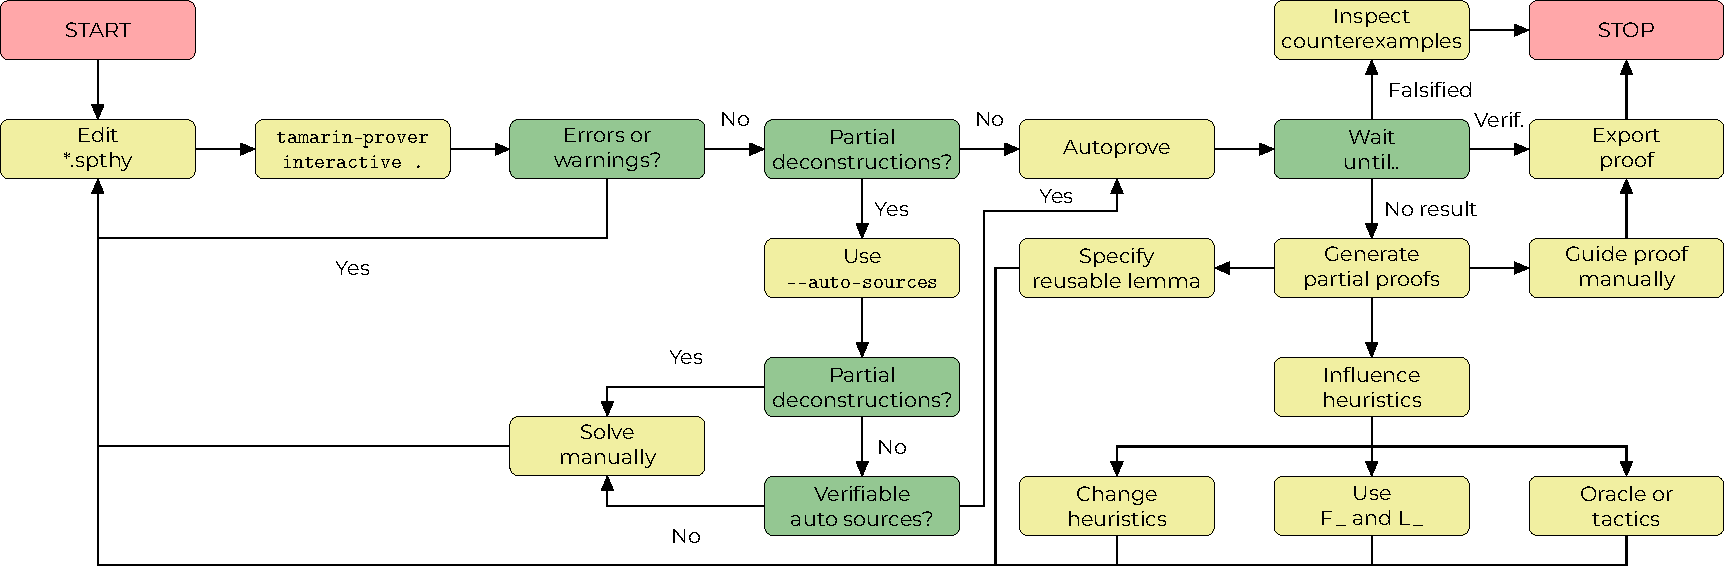
\includegraphics[width=\textwidth]{./figures/lecture_9/workflow_gui}
    \end{figure}
\end{frame}

\begin{frame}[fragile]{This lecture}
    \tableofcontents
\end{frame}

% ---------------------------------------------------------------------------- %

\section{Custom Threat Models}

% ---------------------------------------------------------------------------- %

\begin{frame}[fragile]{Threat model}
    \begin{itemize}
        \item \textbf{Threat model}: Adversary capabilities
        \item So far, we have considered the default \textbf{Dolev-Yao} 
              adversary model
        \begin{itemize}
            \item All messages are sent to the attacker who can either
                  \textbf{drop}, \textbf{modify}, or \textbf{forward} them
            \item When the attacker learns a cryptographic key, it can perform 
                  cryptographic operations to add new messages to its knowledge 
                  set
            \item However, it cannot forge or read cryptographically protected 
                  messages \textbf{without knowing the corresponding keys}
        \end{itemize}
        \item In practice, we often want to consider a \textbf{stronger} or 
              \textbf{weaker} adversary model
    \end{itemize}
\end{frame}

\begin{frame}[fragile]{Choosing a threat model}
    \begin{itemize}
        \item Deciding on a realistic or ``correct'' threat model is not always 
              easy
        \item If the specification of the protocol you are modeling does not 
              explicitly state the threat model, try to determine the
              \textbf{weakest attacker} required to break the system
        \begin{itemize}
            \item A protocol proven secure against a strong attacker is also 
                  secure against a weaker attacker
        \end{itemize}
        \item When writing models:
        \begin{itemize}
            \item If you find attacks: \textbf{Weaken} the attacker
            \item If you cannot find attacks: \textbf{Strengthen} the attacker
        \end{itemize}
    \end{itemize}
\end{frame}

\begin{frame}[fragile]{Modeling corrupted users}
    \begin{itemize}
        \item We strengthen the attacker by adding rules that
              \textbf{reveal secrets}
    \end{itemize}
    \begin{center}
        \begin{tabular}{c}
            \begin{lstlisting}[
                style = tamarin,
                numbers = none,
                gobble = 12,
            ]
            rule reveal_session_key:
                [ !SessionKey(A, k) ] --[ Reveal(A) ]-> [ Out(k) ]
            \end{lstlisting}
        \end{tabular}
    \end{center}
    \begin{itemize}
        \item In lemmas, we can exclude obvious attacks by ignoring traces 
              where the attacker directly learns some value
    \end{itemize}
    \begin{center}
        \begin{tabular}{c}
            \begin{lstlisting}[
                style = tamarin,
                numbers = none,
                gobble = 12,
            ]
            lemma session_key_secrecy:
                " All A k #i . Secret(A, k)@i
                    ==> not (Ex #r . K(k)@r)
                          | (Ex #r . Reveal(A)@r) "
            \end{lstlisting}
        \end{tabular}
    \end{center}
    \begin{itemize}
        \item Sometimes we might want to check whether a property still holds 
              even after one or more parties have been compromised
    \end{itemize}
\end{frame}

\begin{frame}[fragile]{Example: PKI}
    \begin{columns}
        \begin{column}{0.55\textwidth}
            \begin{itemize}
                \item Protocols often assume that the sender and receiver know 
                      each other's public keys \textbf{before} the protocol 
                      starts
                \item Instead of modeling the detailed public key 
                      infrastructure, we model it as an
                      \textbf{initialization rule}
                \item We use the reveal rule to let the attacker get access to 
                      key pairs
            \end{itemize}
        \end{column}
        \begin{column}{0.45\textwidth}
            \begin{lstlisting}[
                style = tamarin,
                gobble = 16,
            ]
                functions: pk/1

                /* Create a key pair */
                rule register_pk:
                    let
                        pubkey = pk(~ltk)
                    in
                    [ Fr(~ltk) ]
                  --[ Register($A, ~ltk) ]->
                    [ !Ltk($A, ~ltk)
                    , !Pk($A, pubkey)
                    , Out(pubkey) ]

                /* Reveal the long-term key */
                rule reveal_ltk:
                    [ !Ltk(A, ltk) ]
                  --[ Reveal(A) ]->
                    [ Out(ltk) ]
            \end{lstlisting}
        \end{column}
    \end{columns}
    \begin{tikzpicture}[remember picture,overlay]%
        \draw[ultra thick]
            ($(current page.north west)+(8.7cm, .5cm)$) to
            ($(current page.south west)+(8.7cm, -.5cm)$);
    \end{tikzpicture}%
\end{frame}

\begin{frame}[t,fragile]{Channel types}
    \begin{columns}[T]
        \begin{column}{0.55\textwidth}
            \begin{itemize}
                \item Recall: By default, the attacker has access to all 
                      messages sent by \texttt{Out()}
                \item If we want to \textbf{weaken} the attacker, we can limit 
                      its network access
                \item We can model a new channel that provides:
                \begin{enumerate}
                    \item<1-> authenticity,
                    \item<2-> confidentiality, or
                    \item<3-> a combination of both
                \end{enumerate}
            \end{itemize}
        \end{column}
        \begin{column}{0.45\textwidth}
            \begin{onlyenv}<1>
                \begin{lstlisting}[
                    style = tamarin,
                    gobble = 16,
                ]
                /* Authenticity guarantees the
                   identity of the sender but 
                   allows the attacker to
                   choose the receiver. The
                   channel is not confidential
                   and leaks all messages to
                   the attacker. */

                // Authentic channel: Out
                rule auth_chan_send:
                    [ AuthSend(A,B,m) ]
                  --[ AuthChan_Out(A,B,m) ]->
                    [ !Auth(A,m), Out(m) ]
  
                // Authentic channel: In
                rule auth_chan_receive:
                    [ !Auth(A, m), In(B) ]
                  --[ AuthChan_In(A,B,m) ]->
                    [ AuthRecv(A,B,m) ]
                \end{lstlisting}
            \end{onlyenv}
            \begin{onlyenv}<2>
                \begin{lstlisting}[
                    style = tamarin,
                    gobble = 16,
                ]
                /* Confidentiality guarantees
                   the receiver's identity.
                   The channel does not leak
                   messages but allows the
                   attacker to inject to it. */

                // Confidential channel: Out
                rule conf_chan_send:
                    [ ConfSend(A,B,m) ]
                  --[ ConfChan_Out(A,B,m) ]->
                    [ !Conf(B,m) ]

                // Confidential channel: In
                rule conf_chan_receive:
                    [ !Conf(B, m), In(A) ]
                  --[ ConfChan_In(A,B,m) ]->
                    [ ConfRecv(A,B,m) ]

                // Confidential channel: Inject
                rule conf_chan_inject:
                    [ In(<A,B,m>) ]
                  --[  ]->
                    [ ConfSend(A,B,m) ]
                \end{lstlisting}
            \end{onlyenv}
            \begin{onlyenv}<3>
                \begin{lstlisting}[
                    style = tamarin,
                    gobble = 16,
                ]
                /* A secure channel provides
                   both authenticity and
                   confidentiality. The
                   attacker has no access to
                   any messages sent over
                   the channel and cannot
                   inject messages into it. */

                // Secure channel: Out
                rule sec_chan_send:
                    [ SecSend(A,B,m) ]
                  --[ SecChan_Out(A,B,m) ]->
                    [ !Sec(A,B,m) ]
                
                // Secure channel: In
                rule sec_chan_receive:
                    [ !Sec(A,B,m) ]
                  --[ SecChan_In(A,B,m) ]->
                    [ SecRecv(A,B,m) ]
                \end{lstlisting}
            \end{onlyenv}
        \end{column}
    \end{columns}
    \begin{tikzpicture}[remember picture,overlay]%
        \draw[ultra thick]
            ($(current page.north west)+(8.7cm, .5cm)$) to
            ($(current page.south west)+(8.7cm, -.5cm)$);
    \end{tikzpicture}%
\end{frame}

% ---------------------------------------------------------------------------- %

\section{A Hierarchy of Authentication Properties}

% ---------------------------------------------------------------------------- %

\begin{frame}[fragile]{Lowe's hierarchy}
    \begin{itemize}
        \item In the literature, you will see multiple variations of 
              authentication claims with subtle differences
        \item In 1997, Gavin Lowe proposed
              \textbf{a hierarchy of authentication properties} in increasing 
              strength:
        \begin{enumerate}
            \item aliveness,
            \item weak agreement,
            \item non-injective agreement, and
            \item injective agreement
        \end{enumerate}
        \item Each property applies from either party's perspective
    \end{itemize}
\end{frame}

\begin{frame}[fragile]{Authentication claims}
    \begin{columns}[T]
        \begin{column}{.65\textwidth}
            We typically use the following action facts:
            \begin{itemize}
                \item \texttt{Create(X)} -- Create Agent X
                \item \texttt{Running(X,Y,t)} -- Agent X believes to be 
                      executing the protocol with agent Y and has learned term t
                \item \texttt{Commit(X,Y,t)} -- Agent X believes to be have 
                      completed the protocol with agent Y and has learned term t
                \item \texttt{Reveal(X)} -- Agent X has revealed its long-term 
                      secret(s)
            \end{itemize}
        \end{column}
        \begin{column}{.35\textwidth}
            \begin{figure}
                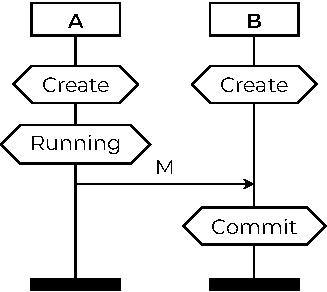
\includegraphics[width=.75\textwidth]
                    {./figures/lecture_7/authentication_claims_1}\\[.5cm]%
                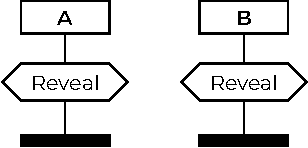
\includegraphics[width=.75\textwidth]
                    {./figures/lecture_7/authentication_claims_2}
            \end{figure}
        \end{column}
    \end{columns}
    \begin{tikzpicture}[remember picture,overlay]%
        \draw[ultra thick]
            ($(current page.north west)+(10.2cm, .5cm)$) to
            ($(current page.south west)+(10.2cm, -.5cm)$);
    \end{tikzpicture}%
\end{frame}

\begin{frame}[fragile,t]{Aliveness}
    A protocol guarantees \textbf{aliveness}\\ to an agent \textit{a} in role 
    \textit{A} if, whenever \textit{a} completes a run of the protocol, 
    seemingly with \textit{b} in role \textit{B}, then \textit{b} has 
    previously been running the protocol.
    \vfill
    \begin{center}
        \begin{tabular}{c}
            \lstinputlisting [
                style = tamarin,
                firstline = 13,
                lastline  = 20,
            ] {./models/lowe_hierarchy.spthy}
        \end{tabular}
    \end{center}
\end{frame}

\begin{frame}[fragile,t]{Weak agreement}
    A protocol guarantees \textbf{weak agreement}\\ to an agent \textit{a} in 
    role \textit{A} if, whenever \textit{a} completes a run of the protocol, 
    seemingly with \textit{b} in role \textit{B}, then \textit{b} has 
    previously been running the protocol, \textcolor{red}{seemingly with
    \textit{a}}.
    \vfill
    \begin{center}
        \begin{tabular}{c}
            \lstinputlisting [
                style = tamarin,
                firstline = 22,
                lastline  = 29,
            ] {./models/lowe_hierarchy.spthy}
        \end{tabular}
    \end{center}
\end{frame}

\begin{frame}[fragile,t]{Non-injective agreement}
    A protocol guarantees \textbf{non-injective agreement}\\ to an agent
    \textit{a} in role \textit{A} if, whenever \textit{a} completes a run of 
    the protocol, seemingly with \textit{b} in role \textit{B}, then \textit{b} 
    has previously been running the protocol \textcolor{red}{in role
    \textit{B}}, seemingly with \textit{a}, \textcolor{red}{and they both agree 
    on the term \textit{t}}.
    \vfill
    \begin{center}
        \begin{tabular}{c}
            \lstinputlisting [
                style = tamarin,
                firstline = 31,
                lastline  = 38,
            ] {./models/lowe_hierarchy.spthy}
        \end{tabular}
    \end{center}
\end{frame}

\begin{frame}[fragile,t]{Injective agreement}
    A protocol guarantees \textbf{injective agreement}\\ to an agent \textit{a} 
    in role \textit{A} if, whenever \textit{a} completes a run of the protocol, 
    seemingly with \textit{b} in role \textit{B}, then \textit{b} has 
    previously been running the protocol in role \textit{B}, seemingly with 
    \textit{a}, and they both agree on the term \textit{t}.
    \textcolor{red}{Each run of agent \textit{a} in role \textit{A} corresponds 
    to a unique run of agent \textit{b}.}
    \vfill
    \begin{center}
        \begin{tabular}{c}
            \lstinputlisting [
                style = tamarin,
                firstline = 40,
                lastline  = 49,
            ] {./models/lowe_hierarchy.spthy}
        \end{tabular}
    \end{center}
\end{frame}

% ---------------------------------------------------------------------------- %

\section{Lemma Annotations}

% ---------------------------------------------------------------------------- %

\begin{frame}[fragile]{Lemma annotations}
    \begin{itemize}
        \item Lemma annotations are used to give Tamarin information about how 
              to solve lemmas
        \item Helps \textbf{avoid non-termination} and \textbf{speed up proofs}
        \item Using the incorrect annotations might have the opposite effect
        \item Declared in square brackets after the name of the lemma:
           \hspace*{.5cm}\verb|lemma example [annotation_1, annotation_2, ...]:|
        \item Today: \textbf{induction} and \textbf{reuse}
        \begin{itemize}
            \item Next lecture: sources
        \end{itemize}
    \end{itemize}
\end{frame}

\begin{frame}[fragile]{Motivating example}
    \begin{itemize}
        \item Consider the following model:
    \end{itemize}
    \hspace*{.7cm}
    \begin{tabularx}{.925\linewidth}{c}
        \toprule
        \lstinputlisting [
            style = tamarin,
        ] {./models/loop.spthy}\\
        \bottomrule
    \end{tabularx}
    \begin{itemize}
        \item If you try to verify either lemma with Tamarin's default 
              heuristic, it will cause an infinite loop. \textbf{Why?}
    \end{itemize}
\end{frame}

\begin{frame}[fragile]{Reasoning about loops}
    \begin{columns}
        \begin{column}{0.6\textwidth}
            \begin{itemize}
                \item Our protocol consists of three rules:
                \begin{table}[]
                    \vspace*{.2cm}
                    \small
                    \raggedright
                    {\setbeamercolor{alerted text}{fg=red}
                    \begin{tabular}{lcl}
                        \texttt{Loop}
                        & := &
                            $\mathsf{\left\{\;
                                \alert<0>{\dfrac{Fr(\tildelow{}x)}{A(x)}{}[Start(x)]}
                            \;\right\}}$ \\[4mm]
                        & $\cup$ &
                            $\mathsf{\left\{\;
                                \alert<2-6>{\dfrac{A(x)}{A(x)}{}[Loop(x)]}\hspace*{.42cm}
                            \right\}}$ \\[4mm]
                        & $\cup$ &
                            $\mathsf{\left\{\;
                                \alert<0>{\dfrac{A(x)}{}{}[Stop(x)]}\hspace*{.42cm}
                            \;\right\}}$ \\[4mm]
                    \end{tabular}}
                \end{table}
                \item How would Tamarin reason backwards from the action fact 
                      \texttt{Loop(X)} to find a counterexample?
            \end{itemize}
        \end{column}
        \begin{column}{0.4\textwidth}
            \begin{figure}
                \includegraphics<1>[height=.85\textheight]
                    {./figures/lecture_7/loop_dependency_graph_0}%
                \includegraphics<2>[height=.85\textheight]
                    {./figures/lecture_7/loop_dependency_graph_1}%
                \includegraphics<3>[height=.85\textheight]
                    {./figures/lecture_7/loop_dependency_graph_2}%
                \includegraphics<4>[height=.85\textheight]
                    {./figures/lecture_7/loop_dependency_graph_3}%
                \includegraphics<5>[height=.85\textheight]
                    {./figures/lecture_7/loop_dependency_graph_4}%
                \includegraphics<6>[height=.85\textheight]
                    {./figures/lecture_7/loop_dependency_graph_5}%
            \end{figure}
        \end{column}
    \end{columns}
    \begin{tikzpicture}[remember picture,overlay]%
        \draw[ultra thick]
            ($(current page.north west)+(10cm, .5cm)$) to
            ($(current page.south west)+(10cm, -.5cm)$);
    \end{tikzpicture}%
\end{frame}

\begin{frame}[fragile]{Why not just break the loop?}
    \begin{itemize}
        \item Some protocols, such as TESLA, require looping behavior
        \begin{itemize}
            \item The TESLA protocol is a stream authentication protocol, i.e., 
                  a protocol that authenticates a continuous stream of packets, 
                  broadcast over an unreliable and untrusted medium to a group 
                  of receivers
            \item Modeling the protocol involves repeatedly applying a hash 
                  function on some value to create a \textbf{hash chain}
        \end{itemize}
        \item We want to write generic lemmas and avoid limiting them to a 
              specific number of iterations (e.g., after repeating a step three 
              times, property P should hold)
        \item How do we solve this? \textbf{Induction}
    \end{itemize}
\end{frame}

\begin{frame}[fragile]{Induction}
    \begin{itemize}
        \item Abstractly: Induction on the length of the trace
        \item The hypothesis is assumed for all timepoints, except for the last 
              one
        \item \textbf{Base case:}
        \begin{itemize}
            \item The property holds for the empty trace
        \end{itemize}
        \item \textbf{Induction hypothesis:}
        \begin{itemize}
            \item If it holds for all traces of length $n - 1$, it holds for 
                  the traces of length $n$
            \item Tamarin uses a \textit{last} event: if the property holds 
                  without the \textit{last} event, we want to prove that it 
                  also holds with the \textit{last} event
        \end{itemize}
        \item When using induction, ensure that the hypothesis is strong enough
    \end{itemize}
\end{frame}

\begin{frame}[fragile,t]{Induction}
    \begin{itemize}
        \item Annotation: \texttt{[use\_induction]}
            \vspace*{.5cm}
            \begin{lstlisting} [
                style = tamarin,
                gobble = 16,
                xleftmargin = .5cm,
            ]
                lemma AlwaysStarts [use_induction]:
                    " All x #i . Loop(x)@i ==> Ex #j. Start(x)@j "
            \end{lstlisting}
        \item Can also be chosen from the GUI
        \end{itemize}
        \vfill
        \begin{figure}
            \frame{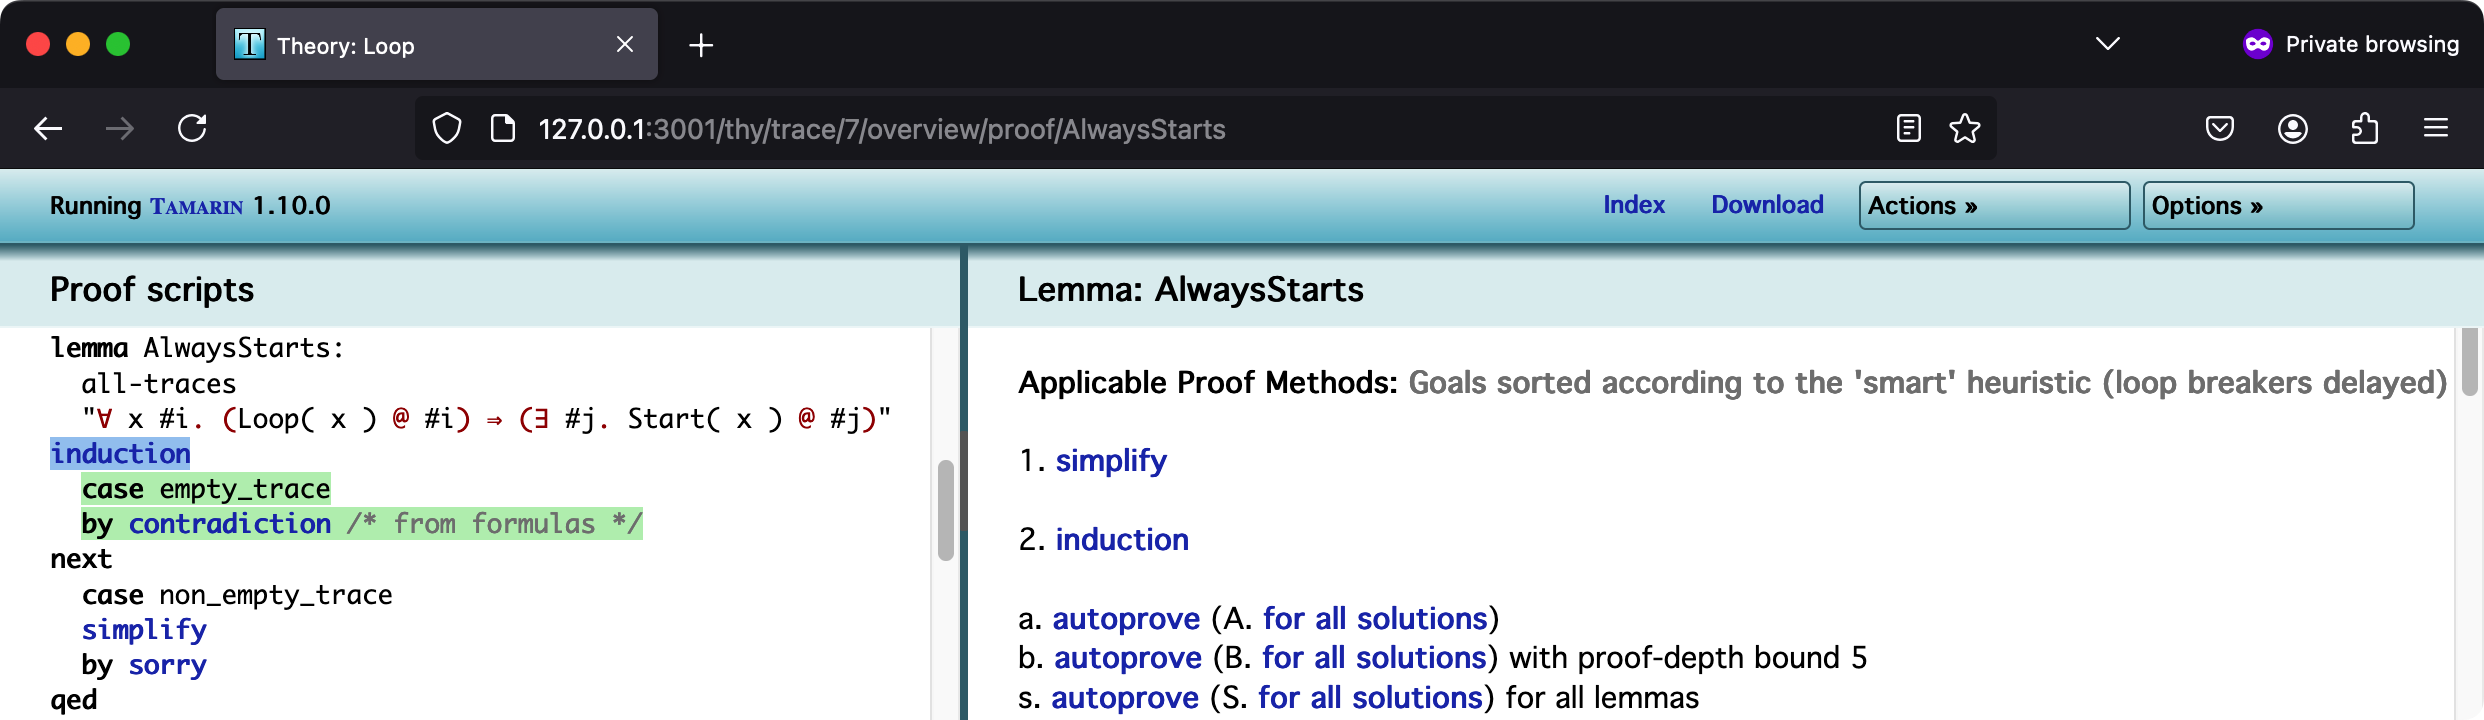
\includegraphics[width=.88\textwidth]
                {./figures/lecture_7/induction_gui}}
        \end{figure}
\end{frame}

\begin{frame}[fragile,t]{Reuse}
    \begin{itemize}
        \item Annotation: \texttt{[reuse]}
        \vspace*{.5cm}
        \begin{lstlisting} [
            style = tamarin,
            gobble = 12,
            xleftmargin = .5cm,
        ]
            lemma AlwaysStarts [use_induction, reuse]:
                " All x #i . Loop(x)@i ==> Ex #j. Start(x)@j "
        \end{lstlisting}
        \item Tells Tamarin to assume that the lemma holds when proving 
              subsequent lemmas
        \item You need to \textbf{make sure that the lemma proves before 
                                  reusing it}
        \begin{itemize}
            \item Tamarin will use it regardless, but the results will be wrong
        \end{itemize}
        \item Does not always reduce proof time
        \begin{itemize}
            \item Use with caution; \textbf{do not mark everything reusable}
            \item We can disable specific reusable lemmas:
                  \texttt{[hide\_lemma=NAME]}
        \end{itemize}
    \end{itemize}
\end{frame}

\begin{frame}[fragile]{Solving the loop problem}
    \begin{itemize}
        \item In the loop example, we first prove that a \texttt{Loop(x)} 
              action is always preceded by a \texttt{Start(x)} action
        \item Then, we reuse the assumption when proving that a
              \texttt{Stop(x)} action is always preceded by a \texttt{Start(x)} 
              action
    \end{itemize}
    \begin{center}
        \begin{tabular}{c}
            \lstinputlisting [
                style = tamarin,
                firstline =  8,
                lastline  = 12,
            ] {./models/loop_fixed.spthy}
        \end{tabular}
    \end{center}
    \begin{itemize}
        \item Including the \texttt{[reuse]} annotation allows Tamarin to 
              assume that the lemma holds for all future proofs
    \end{itemize}
\end{frame}

% ---------------------------------------------------------------------------- %

\section{Predicates and Restrictions}

% ---------------------------------------------------------------------------- %

\begin{frame}[fragile,t]{Predicates}
    \begin{itemize}
        \item It is common to re-use formulas, or parts thereof, across models. 
              To reduce duplication, users can define predicates as
              \textbf{formula shorthands}
        \item A predicate is written as
        \begin{center}
            \verb|predicates: Formula1 <=> Formula2|
        \end{center}    
        which is syntactic sugar for inlining \verb|Formula2| whenever
        \verb|Formula1| is used
        \item For example, we can define a predicate \texttt{Smaller} as
    \end{itemize}
    \begin{center}
        \begin{tabular}{c}
            \begin{lstlisting}[
                style = tamarin,
                gobble = 12,
            ]
            predicates: Smaller(x,y) <=> Ex z. x + z = y
            
            lemma x_smaller_than_y:
                " All x y #i. Compare(x,y)@i ==> Smaller(x,y) "
            \end{lstlisting}
        \end{tabular}
    \end{center}
\end{frame}

\begin{frame}[fragile]{Restrictions}
    \begin{itemize}
        \item Syntactically similar to lemmas, but used to
              \textbf{exclude traces}
        \begin{itemize}
            \item Unlike lemmas, you do \textbf{not} need to prove restrictions
        \end{itemize}
        \item For example, we can define a restriction \texttt{Eq(x,y)}, s.t., 
              whenever it is used, Tamarin will skip any traces where
              \texttt{x} and \texttt{y} are not equal
    \end{itemize}
    \begin{center}
        \begin{tabular}{c}
            \begin{lstlisting}[
                style = tamarin,
                gobble = 12,
            ]
            restriction Equality:
                " All x y #i. Eq(x,y)@i ==> x = y "
            \end{lstlisting}\\
        \end{tabular}
    \end{center}
    \begin{itemize}
        \item This can be used instead of pattern matching for e.g., ensuring 
              that two signatures are equal
    \end{itemize}
    \begin{center}
        \begin{tabular}{c}
            \begin{lstlisting}[
                style = tamarin,
                gobble = 12,
            ]
            rule restriction_example:
                [ In(SignA), In(SignB) ] --[ Eq(SignA, SignB) ]-> [ ]
            \end{lstlisting}\\
        \end{tabular}
    \end{center}
\end{frame}

\begin{frame}[fragile]{Commonly used restrictions}
    \begin{center}
        \begin{tabular}{c}
            \toprule
            \begin{lstlisting}[
                style = tamarin,
                gobble = 12,
            ]
            restriction Unique:
                " All x #i #j. Unique(x)@i & Unique(x)@j ==> #i = #j "

            restriction Equality:
                " All x y #i. Eq(x,y)@i ==> x = y "

            restriction Inequality:
                " All x #i. Neq(x,x)@i ==> F "

            restriction OnlyOnce:
                " All #i #j. OnlyOnce()@i & OnlyOnce()@j ==> #i = #j "

            restriction LessThan:
                " All x y #i. LessThan(x,y)@i ==> x << y "

            restriction GreaterThan:
                " All x y #i. GreaterThan(x,y)@i ==> y << x "
            \end{lstlisting}\\
            \bottomrule
        \end{tabular}
    \end{center}
\end{frame}

\begin{frame}[fragile]{Embedded restrictions}
    \begin{columns}
        \begin{column}{.5\textwidth}
            \begin{itemize}
                \item Embedded restrictions are specified on a per-rule basis 
                      and can use variables within the rule
                \item Use if you only need the restriction in one rule
                \item The examples on the right are functionally equal
            \end{itemize}
        \end{column}
        \begin{column}{.5\textwidth}
            \begin{lstlisting}[
                style = tamarin,
                gobble = 12,
            ]
            /* Only consider traces where
               a is less than b */
            rule embedded_restriction_example:
                [ F(a, b) ]
              --[ _restrict(a << b) ]->
                [  ]
            \end{lstlisting}
            \vspace*{1cm}
            \begin{lstlisting}[
                style = tamarin,
                gobble = 12,
            ]
            /* Only consider traces where
               a is less than b */
            rule restriction_example:
                [ F(a, b) ]
              --[ LessThan(a, b) ]->
                [  ]

            restriction LessThan:
                " All x y #i. LessThan(x,y)@i
                    ==> x << y "
                \end{lstlisting}
        \end{column}
    \end{columns}
    \vsep
\end{frame}

% ---------------------------------------------------------------------------- %
% Reading Material
% ---------------------------------------------------------------------------- %
\begin{frame}[fragile]{Reading material}
    \textbf{Recommended reading}:\\\;
        ~\cite[Ch. 5.9--5.10, 9--10]{tamarin-book},
        ~\cite[Ch. 8.3]{meier2013thesis}
    \begin{refsection}
        \nocite{tamarin-book,meier2013thesis}
        \printbibliography[heading=none]
    \end{refsection}
\end{frame}

\begin{frame}[fragile]{Reading material}
    \textbf{Additional reading}:
        ~\cite{lowe1997hierarchy},
        ~\cite{rfc4082}
    \begin{refsection}
        \nocite{rfc4082,lowe1997hierarchy}
        \printbibliography[heading=none]
    \end{refsection}
\end{frame}
% ---------------------------------------------------------------------------- %

\end{document}
